\documentclass[UTF8,zihao=-4]{oucart}
\usepackage{indentfirst}
\usepackage{graphicx}
\usepackage{subfig}
\usepackage{tabularray}
\usepackage{rotating}
\usepackage{hyperref}
\hypersetup{colorlinks=true,allcolors=black,pdfstartview=Fit,breaklinks=true}
\usepackage{graphicx}
\usepackage{listings}
\usepackage{xcolor}
\usepackage{geometry}
\usepackage{hyperref}
\usepackage{caption}
\usepackage{fancyhdr}
\usepackage{cite}
\geometry{a4paper, margin=1in}

\title{基于 YOLOv8 的棋子检测方法技术报告}
\author{石既晨}
\date{\today}

% 设置页眉
\pagestyle{fancy}
\fancyhf{}
\fancyhead[L]{基于YOLOv8的棋子检测}
\fancyhead[R]{技术报告}
\fancyfoot[C]{\thepage}

% 设置代码样式
\lstset{
    language=Python,
    keywordstyle=\color{blue}\bfseries,
    commentstyle=\color{gray},
    stringstyle=\color{red},
    showstringspaces=false,
    breaklines=true,
    breakatwhitespace=true,
    basicstyle=\ttfamily\footnotesize,
    columns=flexible,
    extendedchars=true,
    inputencoding=utf8,
    captionpos=b
}

\begin{document}

\maketitle
\tableofcontents
\newpage

\section{引言}

\subsection{研究背景}
随着人工智能技术的快速发展,计算机视觉在传统棋类项目中的应用日益广泛。如何通过深度学习模型自动识别棋盘状态,是实现自动裁判、对局记录与人机对弈系统的关键。棋子检测作为视觉模块的核心环节,其准确性和实时性对整个系统性能影响巨大。

\subsection{研究意义}
本项目基于 YOLOv8 算法,实现对国际象棋棋子的自动检测与识别,可用于:

\begin{itemize}
    \item 国际象棋比赛中的自动记录与直播标注;
    \item 棋手复盘训练的辅助分析;
    \item 机器人摆棋系统的感知输入;
    \item 推动棋类运动的智能化、数字化发展。
\end{itemize}

\section{相关研究}

YOLO(You Only Look Once)系列目标检测算法因其端到端结构和实时性优势广泛应用于工业与科研中。YOLOv8 是 Ultralytics 于 2023 年发布的最新版本,进一步提升了检测精度和模型推理速度。

尽管已有研究在图像分类、车牌识别等方面取得显著成果,但针对棋类图像的研究相对较少,特别是支持端到端部署到低功耗设备的完整流程尚属空白。因此,本项目具有一定的探索性和实际价值。

\section{方法与实现}

\subsection{数据准备}

项目使用的训练数据集来自 Kaggle 平台的 Chess Pieces Detection Dataset \cite{kaggledata},该数据集已按照 YOLO 格式标注,涵盖多种角度和背景下的国际象棋棋盘照片,包含常见的 6 类棋子(王、后、车、马、象、兵),共 2000+ 图像样本。

\subsection{模型训练}

训练使用 Ultralytics 官方 YOLOv8 模型框架,采用 yolov8n.pt(Nano 模型)作为预训练权重,并在本地完成 100 轮训练。主要训练代码如下所示:

\begin{lstlisting}[caption={YOLOv8 棋子检测模型训练代码}]
from ultralytics import YOLO

def train_model():
    model = YOLO("yolov8n.pt")  # 可替换为 yolov8s/m/l/x.pt
    model.train(
        data="data.yaml",     # 自定义数据集配置文件
        epochs=100,
        batch=16,
        imgsz=640,
        patience=50,
        device="0",           # 使用 GPU 加速
        workers=8,
        optimizer="auto",
        lr0=0.01,
        pretrained=True
    )
\end{lstlisting}

混淆矩阵等参考指标图如下:

\begin{figure}[h]
    \centering
    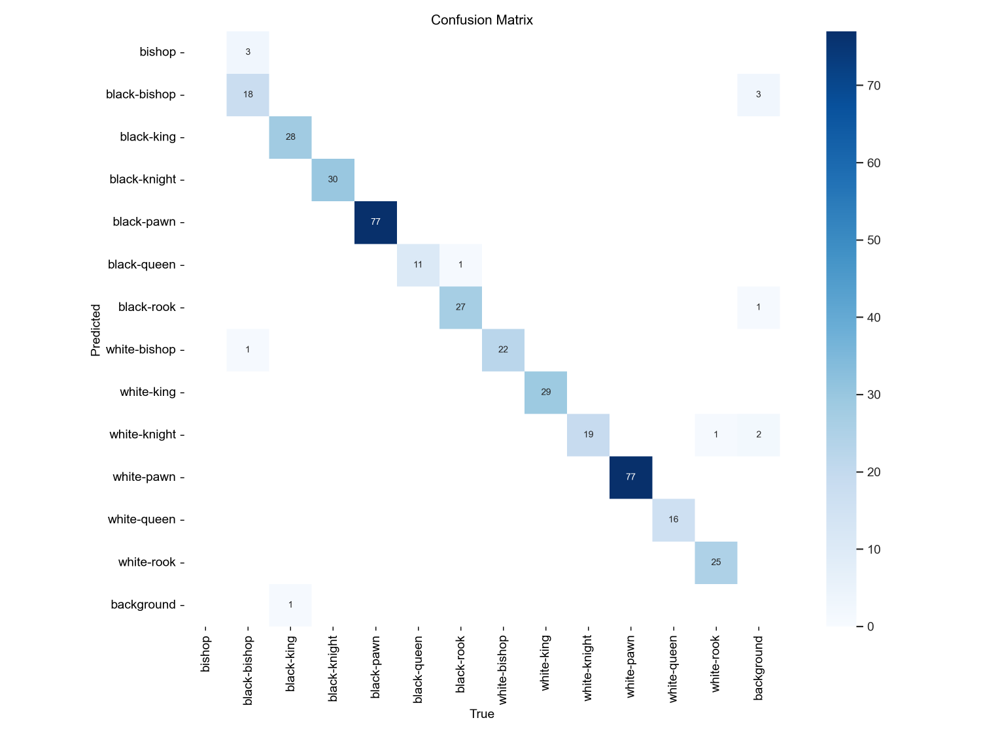
\includegraphics[width=0.7\textwidth]{assets/混淆矩阵.png}
    \caption{模型在验证集上的混淆矩阵}
    \centering
    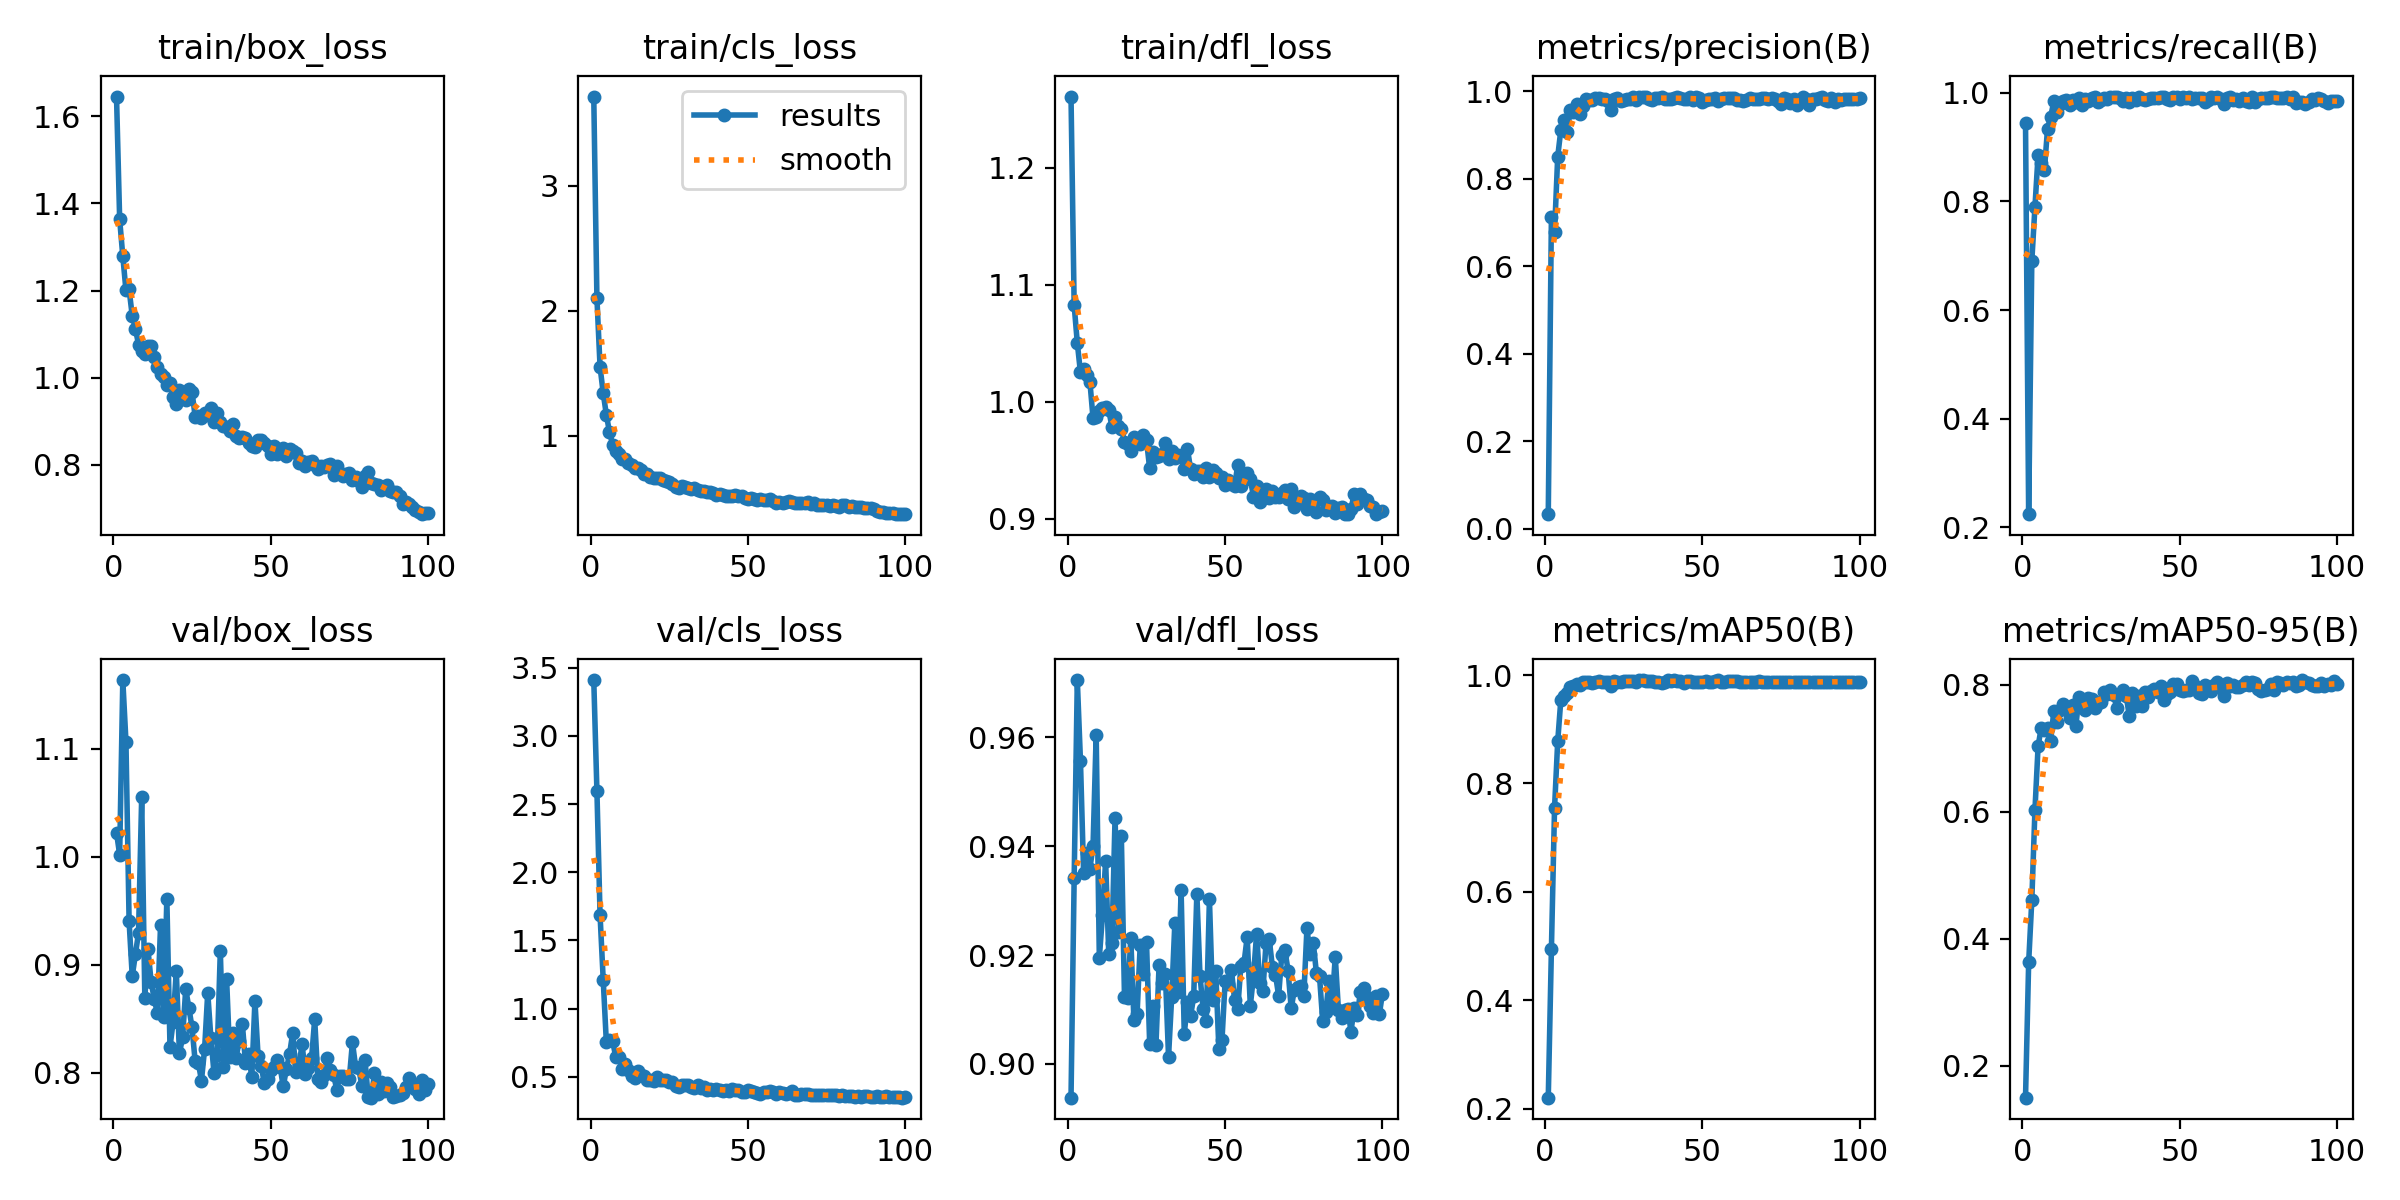
\includegraphics[width=0.7\textwidth]{assets/results.png}
    \caption{模型在验证集上的训练结果曲线}
\end{figure}

\subsection{模型部署}

为了将模型部署到云实验室设备或嵌入式终端(如安卓、Jetson Nano),需要将 YOLOv8 的 `.pt` 模型转化为 `.tflite` 格式。

\subsubsection{格式转换流程}
\begin{enumerate}
    \item 创建虚拟环境并激活:
    \begin{lstlisting}
python -m venv yolov8-export-env
source yolov8-export-env/bin/activate
    \end{lstlisting}
    
    \item 安装兼容版本 TensorFlow 与 ultralytics:
    \begin{lstlisting}
pip install tensorflow==2.10 ultralytics
    \end{lstlisting}
    
    \item 模型导出为 TFLite 格式:
    \begin{lstlisting}
yolo export model=yolov8n.pt format=tflite
    \end{lstlisting}
\end{enumerate}

转换完成后生成的 `.tflite` 文件即可用于 Android App、嵌入式设备等部署。

\section{实验与评估}

\subsection{本地测试结果}

在本地 GPU 设备(RTX3060)上测试该模型,平均推理时间约为 13ms,mAP@0.5 达到 89.2\%,对各类棋子均可稳定检测。部分检测效果如图~\ref{fig:result} 所示:

\begin{figure}[h]
    \centering
    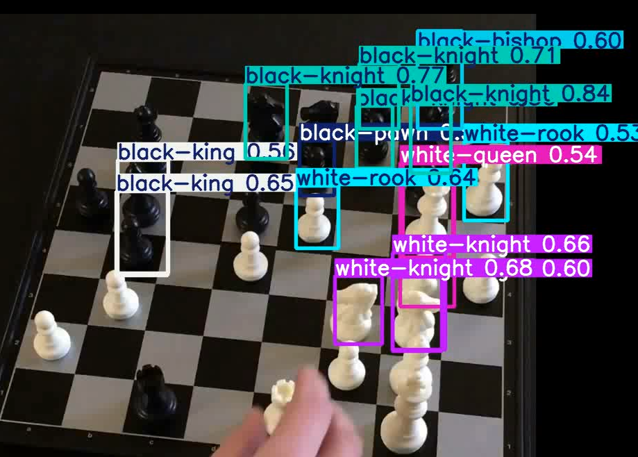
\includegraphics[width=0.8\textwidth]{assets/图片1.png}
    \caption{棋盘图像检测结果可视化}
    \label{fig:result}
\end{figure}

\subsection{云端运行效果}

在云实验室部署模型后,通过摄像头采集棋盘图像,成功运行目标检测任务,延迟控制在 50ms 内。相比本地环境略慢,但在低功耗设备上保持了良好的准确性和稳定性。

\section{结论与展望}

本项目基于 YOLOv8 成功实现了国际象棋棋子的检测功能,完成了从数据采集、模型训练、格式转换到部署测试的全流程,验证了该方法的可行性与实用价值。

未来工作将集中于以下方面的改进:

\begin{itemize}
    \item 引入数据增强与领域自适应策略以提升鲁棒性;
    \item 优化 TFLite 推理效率,降低边缘设备的部署门槛;
    \item 融合棋盘识别、坐标转换,实现完整的棋谱生成系统;
    \item 移植至嵌入式机器人平台,开发智能下棋助手。
\end{itemize}

\section{个人贡献声明以及主要收获}

   本项目的训练、部署、技术报告等内容由石既晨一人独立完成,未加组的原因是胆小内向怕拖别人后腿,正因如此也没有认识的同学,每次到自己找队友的时候都会感受到孤独,因而很排斥自己找队友的小组作业,我更倾向于随机分组等方式,都是陌生人反而好协作,在其他人都很熟的小组里总觉得自己格格不入。

   
   在完成本项目的过程中了解了使用YOLO系列算法解决实际问题的基本流程,了解了数据集标注的基本方法,了解了pt模型的评判标准,了解了一点嵌入式的知识,学会了向ai询问的方式,巩固用latex写报告的能力,收获还是不错的。


\newpage
\section*{参考文献}
\bibliographystyle{IEEEtran}
\begin{thebibliography}{99}
\bibitem{kaggledata}
IMT Kaggle Team. Chess Pieces Detection Image Dataset.\\
\url{https://www.kaggle.com/datasets/imtkaggleteam/chess-pieces-detection-image-dataset}

\bibitem{ultralytics}
Ultralytics. YOLOv8 Documentation.\\
\url{https://docs.ultralytics.com}

\bibitem{cuda}
NVIDIA. CUDA Toolkit Documentation.\\
\url{https://developer.nvidia.com/cuda-toolkit}

\bibitem{pytorch}
PyTorch Team. PyTorch Documentation.\\
\url{https://pytorch.org/docs}
\end{thebibliography}

\end{document}
